\part{Behaviour Trees}
\frame{\partpage}

\begin{frame}{Behaviour trees (BTs)}
	\begin{itemize}
		\pause\item A \textbf{hierarchical} model of decision making
		\pause\item Allow \textbf{complex behaviours} to be built up from \textbf{simple components}
		\pause\item Allow for \textbf{more complex} behaviours than FSMs
		\pause\item First used in Halo 2 (2005), now used extensively
		\pause\item Also used in robotics and other non-game AI applications
	\end{itemize}
\end{frame}

\begin{frame}{Using BTs}
	\begin{itemize}
		\pause\item Fairly easy to implement; plenty of resources online
		\pause\item \textbf{Unreal}: an advanced BT system is built in
		\pause\item \textbf{Unity}: numerous free and paid options on the Asset Store
			e.g.\ Behavior Machine, Behavior Designer, Behave, RAIN
	\end{itemize}
\end{frame}

\begin{frame}{BT basics}
	\begin{itemize}
		\pause\item A BT is a \textbf{tree} of \textbf{nodes}
		\pause\item On each game update (i.e.\ each frame), the root node is \textbf{ticked}
			\begin{itemize}
				\pause\item When a node is ticked, it might cause some or all of its \textbf{children} to tick as well
				\pause\item So ticks propagate down the tree from the root
			\end{itemize}
		\pause\item A ticked node returns one of three \textbf{statuses}:
			\begin{itemize}
				\pause\item Success
				\pause\item Running
				\pause\item Failure
			\end{itemize}
		\pause\item ``Running'' status allows nodes to represent operations that \textbf{last multiple frames}
	\end{itemize}
\end{frame}

\begin{frame}{Node types}
	\begin{itemize}
		\pause\item There are \textbf{three main types} of BT node
		\pause\item \textbf{Leaf} nodes
			\begin{itemize}
				\pause\item No children
				\pause\item Represent actions (i.e.\ the AI agent actually doing something)
			\end{itemize}
		\pause\item \textbf{Decorator} nodes
			\begin{itemize}
				\pause\item One child
				\pause\item Modify the execution of the child
			\end{itemize}
		\pause\item \textbf{Composite} nodes
			\begin{itemize}
				\pause\item Control which of the children are executed on each tick
			\end{itemize}
	\end{itemize}
\end{frame}

\begin{frame}{Leaf nodes}
	\begin{itemize}
		\pause\item Represent \textbf{atomic actions}
			\begin{itemize}
				\pause\item I.e.\ actions which can't sensibly be broken down into smaller actions
			\end{itemize}
		\pause\item E.g.\ walk to, crouch, attack, open door
		\pause\item Status:
			\begin{itemize}
				\pause\item Success means ``the action is done''
				\pause\item Failure means ``the action cannot be done''
				\pause\item Running means ``the action is still in progress''
			\end{itemize}
		\pause\item Leaf nodes can also be used to represent \textbf{conditions}
			\begin{itemize}
				\pause\item E.g.\ ``is my health below 10\%?''
				\pause\item Returns success for true, failure for false
			\end{itemize}
		\pause\item Leaf nodes often have \textbf{parameters} to allow for reuse in different situations
	\end{itemize}
\end{frame}

\begin{frame}{Composite nodes: sequence}
	\begin{itemize}
		\pause\item Run each child, in order
		\pause\item If \textbf{any} child returns failure, stop and return failure
		\pause\item If \textbf{all} children return success, stop and return success
	\end{itemize}
	\pause
	{\footnotesize\Tree
		[.\fbox{Sequence}
			[.\fbox{Walk to chest} ]
			[.\fbox{Open chest} ]
			[.\fbox{Pick up loot} ]
			[.\fbox{Close chest} ]
		]
	}
\end{frame}

\begin{frame}{Sequence nodes and conditions}
	\begin{itemize}
		\pause\item A sequence node can be used like an \lstinline{if (cond1 && cond2)} statement
	\end{itemize}
	\pause
	{\footnotesize\Tree
		[.\fbox{Sequence}
			[.\fbox{Is health $< 10$?} ]
			[.\fbox{Am I near cover?} ]
			[.\fbox{Move to cover} ]
			[.\fbox{Use medkit} ]
		]
	}
\end{frame}

\begin{frame}{Composite nodes: selector}
	\begin{itemize}
		\pause\item Run each child, in order
		\pause\item If a child returns failure, move onto the next one
		\pause\item If \textbf{any} child returns success, stop and return success
	\end{itemize}
	\pause
	{\footnotesize\Tree
		[.\fbox{Selector}
			[.\fbox{Open chest} ]
			[.\fbox{Sequence}
				[.\fbox{Unlock chest} ]
				[.\fbox{Open chest} ]
			]
			[.\fbox{Smash chest} ]
		]
	}
\end{frame}

\begin{frame}{Selectors and priority}
	\begin{itemize}
		\pause\item Order of selector children represents the \textbf{priority} of different alternatives
	\end{itemize}
	\pause
	{\scriptsize\Tree
		[.\fbox{Selector}
			[.\fbox{Sequence}
				[.\fbox{Health $<$ 10?} ]
				[.\fbox{Run away} ]
			]
			[.\fbox{Sequence}
				[.\fbox{Player visible?} ]
				[.\fbox{Attack} ]
			]
			[.\fbox{Patrol} ]
		]
	}
\end{frame}

\begin{frame}{Sequence vs selector}
	\begin{itemize}
		\pause\item Sequence: perform a list of actions; if one of them fails then abandon the task
		\pause\item Selector: try a list of alternatives; stop once you find one that works
		\pause\item Sequence works like \lstinline{and}, selector works like \lstinline{or}
	\end{itemize}
\end{frame}

\begin{frame}{Other composite nodes}
	\begin{itemize}
		\pause\item Execute children in \textbf{random} order
		\pause\item Execute children in \textbf{parallel}
		\pause\item Most BT frameworks allow programmers to create custom composite nodes
	\end{itemize}
\end{frame}

\begin{frame}{Decorator nodes}
	\begin{itemize}
		\pause\item \textbf{Inverter}: if child returns success then return failure, and vice versa
		\pause\item \textbf{Repeater}: run the child a number of times, or forever
		\pause\item Most BT frameworks allow programmers to create custom decorator nodes
	\end{itemize}
\end{frame}

\begin{frame}{Blackboard}
	\begin{itemize}
		\pause\item It is often useful to \textbf{share} data between nodes
		\pause\item A \textbf{blackboard} (sometimes called a \textbf{data context}) allows this
		\pause\item Blackboard defines \textbf{variables}, which can be \textbf{read} and \textbf{written} by nodes
		\pause\item Blackboard can be \textbf{local} to the AI agent, \textbf{shared} between several agents, or \textbf{global} to all agents
		\pause\item (Shared blackboards mean that your AI has ``telepathy'' --- this may or may not be desirable!)
	\end{itemize}
\end{frame}

\begin{frame}{BTs in The Division}
	\begin{center}
		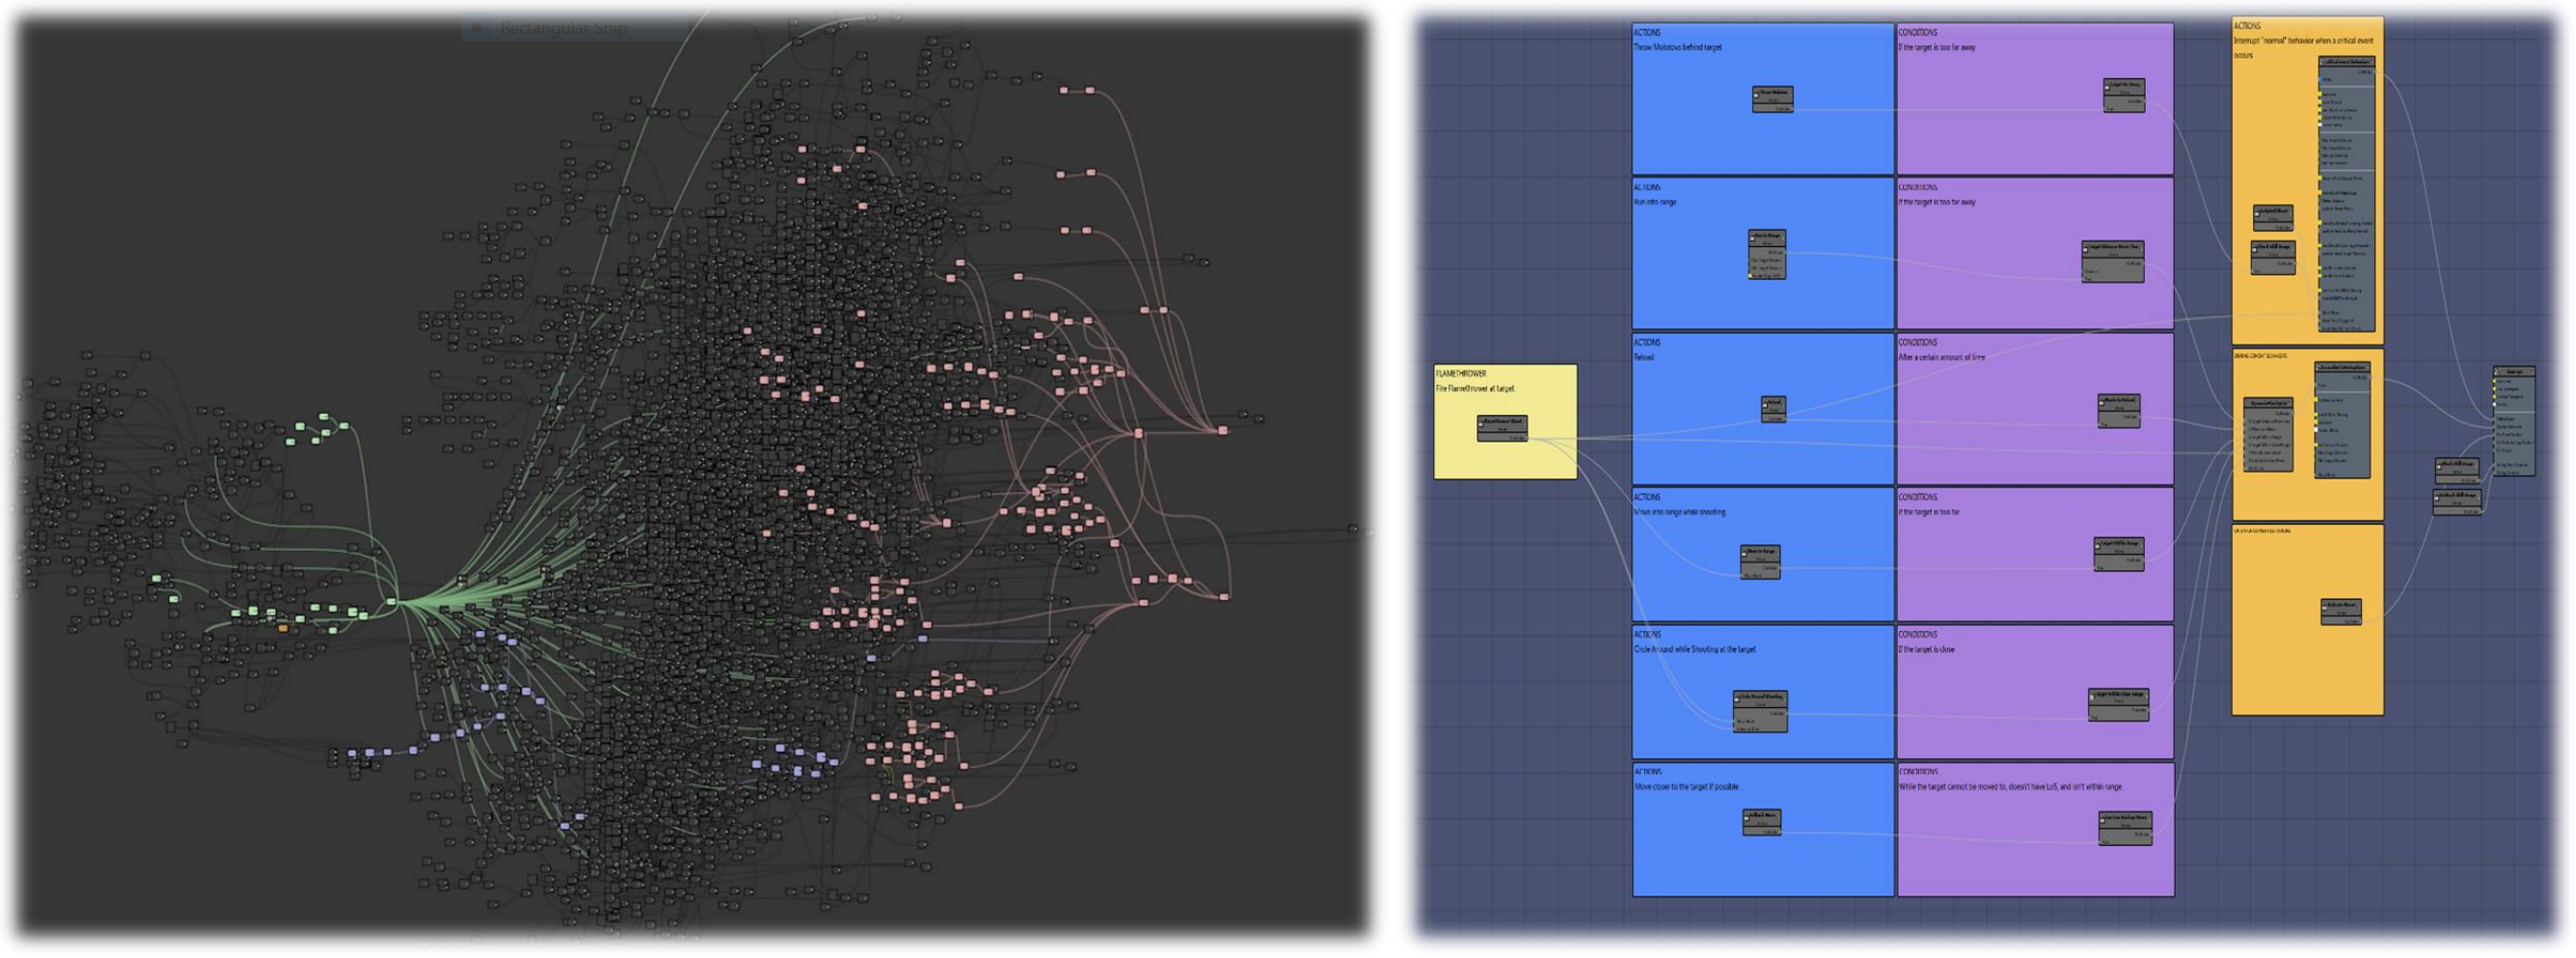
\includegraphics[width=\textwidth]{the_division}
		
		\url{http://www.gdcvault.com/play/1023382/AI-Behavior-Editing-and-Debugging}
	\end{center}
\end{frame}

\begin{frame}{Activity}
	\begin{center}
		\textbf{Unreal users}: follow the tutorial at
		
		\url{https://docs.unrealengine.com/latest/INT/Engine/AI/BehaviorTrees/QuickStart/}
		
		\vspace{2ex}
		
		\textbf{Unity users}: download ``Behaviour Machine Free'' from the Asset Store, and follow the tutorial at
		
		\url{https://youtu.be/ZVl1FM24OXg}
	\end{center}
\end{frame}
